\section{Ejercicio 3}

\subsection{Introducción}

\paragraph{}
El tercer y \'ultimo problema de este trabajo pr\'actico consiste en, dadas dos listas con horarios de entrada y salida de ciertos trabajadores a una empresa, decidir cu\'al es el mayor n\'umero de los mismos que se encuentran al mismo tiempo dentro de dicha empresa.

\paragraph{}
En una primer mirada, se pens\'o que la mejor forma de resolver el ejercicio era aplicando un algoritmo similar al del quicksort\footnote{Alguna referencia que explique el algoritmo}, s\'olo que el mismo se realizaba sobre conjuntos y no sobre arreglos. En resumidas cuentas, la idea era tomar un trabajador cualquiera del grupo, y separar en tres conjuntos distintos: los que se cruzaban con el trabajador pivote, los que sal\'ian antes que el pivote entrara y los que entraban luego que el pivote saliera\footnote{Para que el algoritmo funcionara bien, se deb\'ia tener cierto cuidado con los trabajadores que se cruzaran con el pivote, pero la explicaci\'on de estos detalles no hacen a la escencia de la introducci\'on. Adem\'as, este algoritmo fue descartado m\'as adelante, por lo que estos detalles son irrelevantes para este trabajo.}. De esta manera, si se repet\'ia el proceso varias veces, se llegaba a tener varios conjuntos en los cuales aparec\'ian solamente trabajadores que se cruzaban en sus horarios dentro de la empresa. Finalmente, s\'olo restaba devolver el mayor cardinal de dichos conjuntos.

\paragraph{}
Al igual que el quicksort, si el pivote era elegido al azar, el algoritmo anterior contaba con una complejidad promedio de \Ode{n*log(n)} (donde $n$ es la cantidad de trabajadores).  Igualmente, el peor caso segu\'ia siendo \Ode{n^2}, por lo que no se iba a poder respetar la cota dada como m\'axima para este trabajo, ya que se especificaba que el algoritmo deb\'ia tener una complejidad menor a \Ode{n^2}.

\paragraph{}
Pero luego de un mejor an\'alisis del problema, se cay\'o en la cuenta que los datos de entrada contaban con la caracter\'istica de estar ordenados por horario (tanto los de entrada como los de salida), por lo que inmediatamente surgi\'o la idea de poder solucionar el problema con una complejidad de \Ode{n}.

\paragraph{}
Para lograr dicha soluci\'on, no se requiri\'o de una t\'ecnica compleja. En realidad, lo que se hizo fue iterar sobre las dos listas de entrada, que conten\'ian los horarios de entrada y de salida de los trabajadores. De esta forma, con un recorrido lineal sobre ambas listas de entrada, se pod\'ia saber con certeza cu\'al era la respuesta al problema para las mismas.


\subsection{Explicación}
\label{explicacion}

\paragraph{}
Para encontrar soluci\'on al problema dado, lo primero que se realiz\'o fue pensar qu\'e cosas se necesitaban para representarlo. Para ello se cre\'o una clase ``Empresa'', la cual consta de dos arreglos que contienen en cada posici\'on, una hora junto con un nombre de un trabajador, ambos arreglos ordenados ascendentemente por hora. Uno de ellos contiene los horarios de entrada de los trabajadores, mientras que el otro contiene los de salida. Adem\'as, se cuenta con las siguientes precondiciones:
\begin{itemize}
 \item Cada trabajador ingresa estrictamente antes de egresar
 \item Los horarios van desde 00:00:00 hasta 23:59:59.
\end{itemize}
 

\paragraph{}
Una vez cargados los datos en nuestra estructura, se procedi\'o a armar el algoritmo que resuelve el problema. La idea del mismo fue ir index\'ando ambos arreglos desde la posici\'on 0 hasta la n-1 \'esima. De esta forma, lo que se hizo fue ir recorriendo el arreglo que conten\'ia los horarios de entrada, hasta que se encontrara una posici\'on en la cu\'al su horario de entrada fuese mayor al horario de salida que se estaba indexando en ese momento (en el caso de la primer iteraci\'on por ejemplo, el horario ubicado en la posici\'on 0 del arreglo de horarios de salida). Mientras se realizaba esto, un contador con valor inicial 0 se iba incrementando con cada iteraci\'on, simulando as\'i la cantidad de trabajadores que iban entrando.

\paragraph{}
Cuando se encontraba un horario de entrada mayor al de salida esto significaba que, antes de que ingresara un nuevo trabajador, al menos uno se hab\'ia retirado, por lo que se sal\'ia de esta iteraci\'on. En un primer paso se verificaba cu\'antos trabajadores habían entrado hasta ese momento y se guardaba en una variable (siempre y cuando dicho valor fuese mayor al guardado anteriormente). Luego, se recorr\'ia el arreglo que conten\'ia los horarios de salida de la misma manera que antes: recorrer hasta que se encuentre un horario mayor al indexado en el arreglo de entradas, con la diferencia que en este caso, cada vez que se iteraba, se decrementaba el contador de trabajadores simulando un egreso.

\paragraph{}
Esto se repet\'ia varias veces, hasta que se indexaran todas las posiciones del arreglo de los horarios de entrada, devolviendo finalmente el valor que se iba actualizando tras cada cambio de iteraci\'on, es decir, el valor que se actualizaba una vez que se dejaba de iterar el arreglo con los horarios de entrada.

\paragraph{}
A modo de una explicaci\'on m\'as clara que nos acerque un poco m\'as a la implementaci\'on, detallamos lo expreso anteriormente a trav\'es del siguiente pseudoc\'odigo:

\incmargin{1em}
\linesnumbered
\restylealgo{boxed}
%\dontprintsemicolon


\SetKw{Orden}{Complejidad:}
\begin{algorithm}[H]
\Orden{O(n)}
\BlankLine
\textbf{var} i,j,maxJuntos,juntosPorAhora : \entero \\
\textbf{var} termine : bool \\
\BlankLine
i $\leftarrow$ j $\leftarrow$ maxJuntos $\leftarrow$ juntosPorAhora $\leftarrow$ 0\tcp*{O(1)}
termine $\leftarrow$ false\tcp*{O(1)}
\BlankLine
\While{(!termine)\tcp*{O(n)}}{

    \While{(noLlegueAlFinal(i,n) $\&\&$ hora(entradas[i]) $\leq$ hora(salidas[j]))\tcp*{O(1)}}{
    
	juntosPorAhora++		\tcp*{O(1)}
	i++				\tcp*{O(1)}
    }
    \BlankLine
    termine = i $\geq$ n			\tcp*{O(1)}
    \BlankLine
    \If{(maxJuntos $\leq$ juntosPorAhora)\tcp*{O(1)}}{maxJuntos $\leftarrow$ juntosPorAhora\tcp*{O(1)}}
    \BlankLine
    \While{(!termine $\&\&$ hora(salidas[j]) $\leq$ hora(entradas[i]))\tcp*{O(1)}}{
    
	juntosPorAhora$--$		\tcp*{O(1)}
	j++						\tcp*{O(1)}
    }

}
\BlankLine
\textbf{return} maxJuntos
\end{algorithm}

\paragraph{}
De esta explicación y de un análisis más minucioso del pseudocódigo, se desprenden algunas hipótesis.
\begin{itemize}
	\item La complejidad temporal del algoritmo es \Ode{n}
	\item El peor caso se da cuando hay muchos trabajadores dispersos durante todo el día. Esto es, por ejemplo, que desde el comienzo del día hasta el final, pase que cada vez que sale un trabajador inmediatamente en ese momento ingrese otro. Esto haría que se ejecute cada while anidado una sola vez por cada iteración.
\end{itemize}


\subsection{Análisis de la complejidad del algoritmo}

\paragraph{}
Para realizar el análisis de la complejidad del algoritmo, se decidió utilizar el modelo uniforme y no el logarítmico. Esto se debió a que en este caso, no resulta lógico evaluar la complejidad de acuerdo al costo de representar los valores de los parámetros de entrada. Más aún, por la forma y el contexto del problema y por el algoritmo implementado para la resolución, no sería correcto hacer un análisis logarítmico ya que en este caso las horas representables están acotadas (habíamos dicho que se encontraban entre 00:00:00 y 23:59:59) y la cantidad de trabajadores, aunque no está explícitamente acotada, podríamos suponerla así. De esta manera, sería válido considerar que la complejidad espacial de cada elemento es unitaria, haciendo inadecuado analizar la complejidad del algoritmo con el modelo logarítmico.

\paragraph{}
Con el objetivo de realizar un mejor análisis de la complejidad del algoritmo propuesto, vamos a analizar el mismo remitiéndonos al pseudocódigo citado en la sección [\ref{explicacion}].

\paragraph{}
Si hacemos una mirada mas minuciosa sobre el pseudocódigo, veremos que la complejidad del algoritmo está dada por $n$, que hace referencia a la cantidad de trabajadores de la empresa. Si vemos las complejidades de cada operación, vemos que todas son constantes, con excepción del flujo ``while'' más grande (aquél que tiene como condición: (!\textit{termine}) ). Veamos por qué sucede esto.

\paragraph{}
Como se puede ver en la línea 5, el booleano \textit{termine} es inicializado con el valor de verdad \false. La otra variable que nos va a interesar para este análisis es \textit{i}, la cuál se inicializa con el valor 0. Con estos valores, y sabiendo que el flujo while que estamos analizando tiene como condición la negación de \textit{termine}, se desprende que el algoritmo terminara sí y solo sí \textit{termine} tome el valor de verdad \true .

\paragraph{}
Si vemos la línea 13 del pseudocódigo, vemos que aquí es modificado el valor de verdad de \textit{termine} y no se modifica en ningún otro lugar. En esta línea se ve que:
\begin{equation}
termine \leftarrow i \geq n
\end{equation}

Entonces, juntando esto con lo dicho anteriormente, se ve claramente que el algoritmo va a finalizar una vez que \textit{i} \ensuremath{\geq} n. Veamos entonces cómo se comporta \textit{i} a lo largo del programa.

\paragraph{}
La variable \textit{i} sólo es modificada en el primer while anidado, y en esta modificación, \textit{i} es incrementada de a uno por vez. Por lo tanto, una vez que se ejecute el contenido de este while anidado n veces, el algoritmo finalizará.

\paragraph{}
Si consideramos la precondición de que todos los trabajadores ingresan a la empresa estrictamente antes de egresar, podemos ver entonces que este primer while anidado va a ejecutarse siempre a lo sumo n veces\footnote{Ver condición del primer while anidado}. Por lo tanto, el algoritmo tiene una complejidad de \Ode{n}.



\subsection{Detalles de Implementación}

\paragraph{}
Para compilar este programa, se debe referir a la carpeta que contiene al ejercicio nº 3 y ejecutar make en consola.

\paragraph{}
Luego de ejecutar make, se creara un archivo ejecutable, llamado main. Para ejecutarlo, se debe hacer una llamada desde la consola respetando el siguiente formato:\\
\texttt{main [nombreEntrada] [nombreSalida]}.

\paragraph{}
Los parámetros son opcionales, pero se puede elegir entre no pasar ningún parámetro, o pasar 2. Si no se pasan parámetros, el programa tomara los valores por defecto, esto quiere decir que el archivo de entrada será el designado por la materia.


\subsection{Resultados}
\label{resultadosej3}

\begin{table}[ht] %ubicacion de la tabla
\centering %centra la tabla
\begin{tabular}{c}
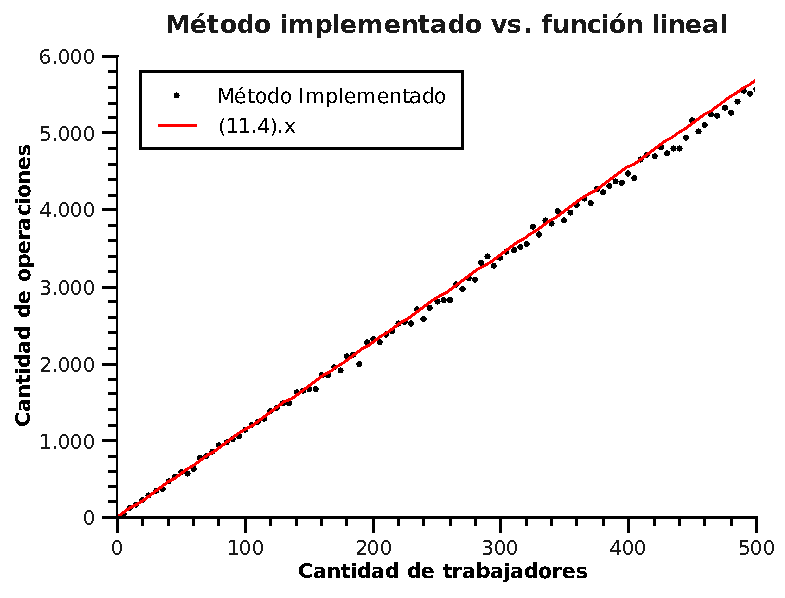
\includegraphics[scale=0.7]{../ej3/graficos/contarOp1.pdf} \\
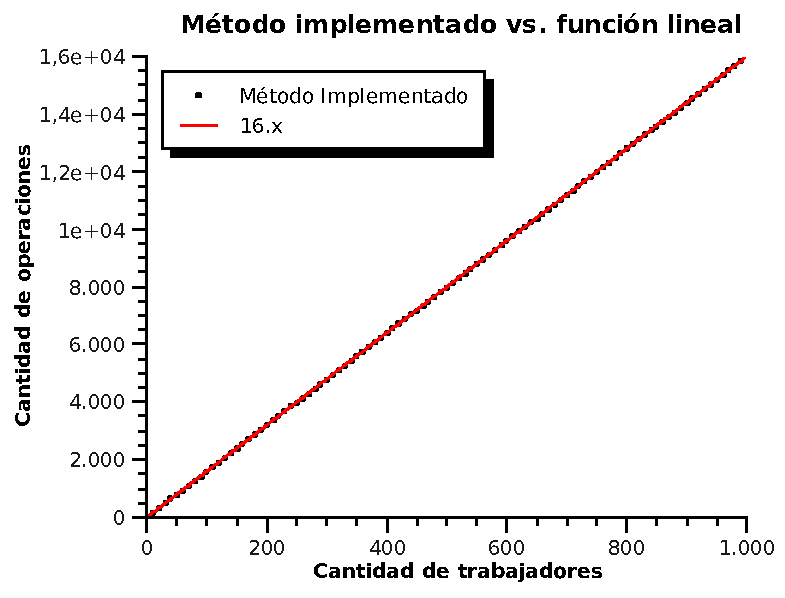
\includegraphics[scale=0.7]{../ej3/graficos/contarOp5.pdf}
\end{tabular}

\caption{Muestran el comportamiento de la cantidad de operaciones contra la cantidad de trabajadores} %titulo de la tabla
\label{cantOp} %con esto puedo referenciar a la tabla \ref{Tiempo metodos}
\end{table}

\begin{table}[ht] %ubicacion de la tabla
\centering %centra la tabla
\begin{tabular}{c}
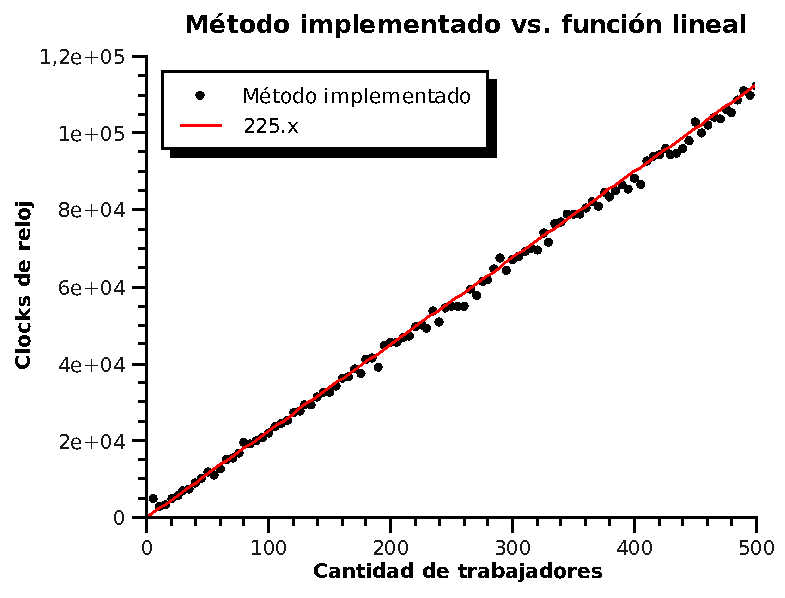
\includegraphics[scale=0.7]{../ej3/graficos/clocks1.pdf} \\
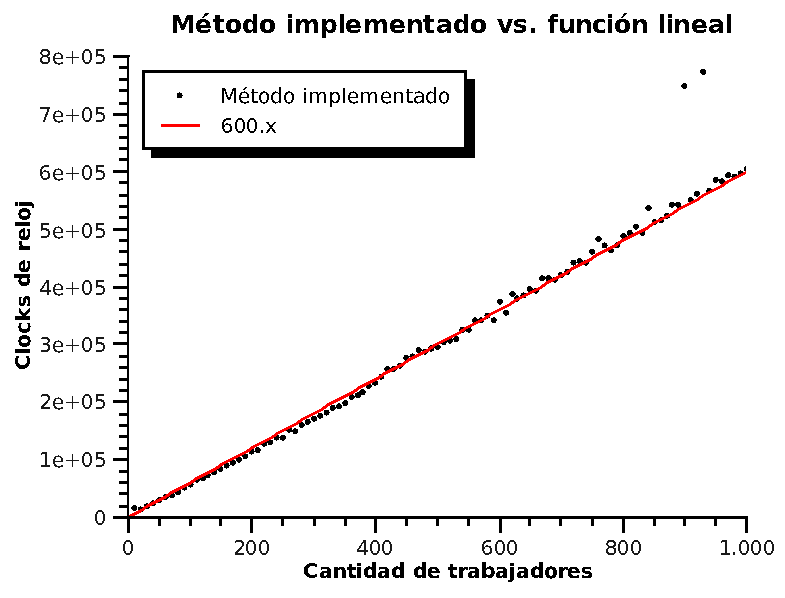
\includegraphics[scale=0.7]{../ej3/graficos/clocks5.pdf}
\end{tabular}

\caption{Muestran el comportamiento de la cantidad de operaciones contra la cantidad de trabajadores} %titulo de la tabla
\label{cantOp} %con esto puedo referenciar a la tabla \ref{Tiempo metodos}
\end{table}

\begin{table}[ht] %ubicacion de la tabla
\centering %centra la tabla
\begin{tabular}{c}
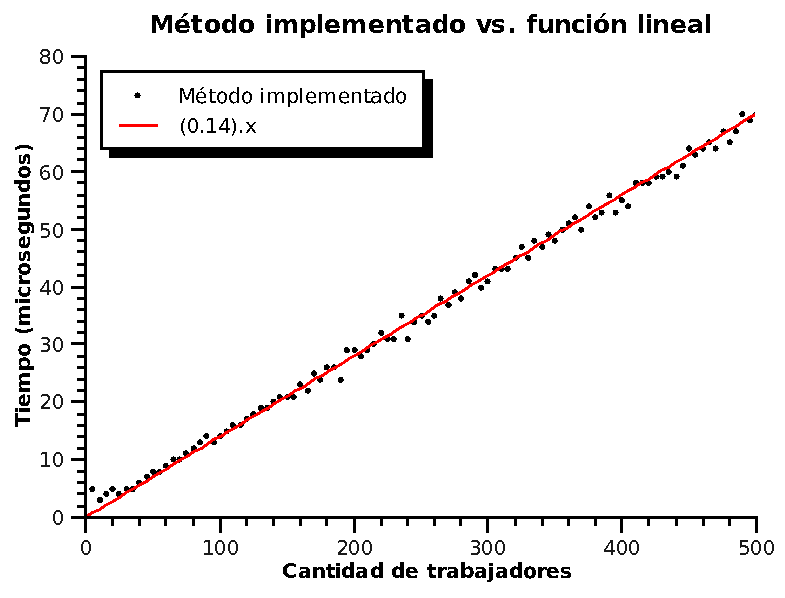
\includegraphics[scale=0.7]{../ej3/graficos/tiempo1.pdf} \\
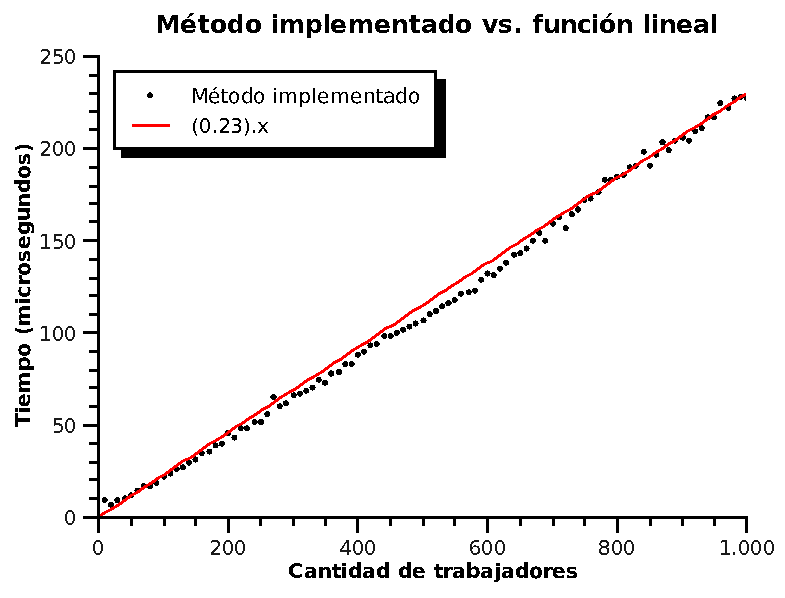
\includegraphics[scale=0.7]{../ej3/graficos/tiempo5.pdf}
\end{tabular}

\caption{Muestran el comportamiento de la cantidad de operaciones contra la cantidad de trabajadores} %titulo de la tabla
\label{cantOp} %con esto puedo referenciar a la tabla \ref{Tiempo metodos}
\end{table}


\subsection{Debate}
\paragraph{}
Como podemos observar en los gráficos propuestos en la sección [\ref{resultadosej3}] en general la implementación realizada se comporta como se esperaba que en teoría funcionara. Es decir, durante el desarrollo del informe sobre este ejercicio, entre otras cosas, hicimos notar que nuestra hipótesis sobre la complejidad del algoritmo era que el mismo tenía un costo de \Ode{n}, donde $n$ es la cantidad de trabajadores de la empresa.

\paragraph{}
Se puede identificar en cada gráfico una marcada similitud entre los resultados arrojados en las distintas mediciones que se hicieron sobre la implementación y alguna recta (o función lineal) , variando esta última su pendiente. Esta pendiente podría compararse o considerarse como la constante que acompa\~na a la complejidad del algoritmo.

\paragraph{}
Se puede notar claramente que esta constante o pendiente, es notablemente mayor en aquellos gráficos en los cuales se evaluó el comportamiento del algoritmo en el peor caso que en los que se evaluó el mismo con entradas al azar.

\paragraph{}
En el gráfico [clocks5] podemos notar dos casos de outliers. Si observamos más detalladamente podemos ver que estos casos se dan con valores de $n$ grandes. Esto puede deberse a que, como el algoritmo tarda más en terminar, es más probable que haya alguna interrupción que irrumpa durante el mismo haciendo que la medición no sea precisa. Esto se debe a la forma en que se miden los ciclos de reloj. Lo que se hace es obtener los ciclos de reloj transcurridos hasta antes de hacer la llamada al algoritmo implementado, luego se toma la misma medición y, finalmente, se toma la diferencia entre ambas mediciones obteniendo como resultado la cantidad de ciclos insumidos por el algoritmo. Pero si durante el algoritmo, una llega una interrupción y la atención de la misma le insume al procesador varias instrucciones, esto puede llegar a provocar una medición de ciclos de reloj muy imprecisa.\\
Más aún, si tomamos en cuenta cómo un sistema operativo hace manejo de los procesos, puede haber llegado a ocurrir que durante la ejecución del algoritmo, este haya consumido todo su tiempo de ejecución asignado por el sistema, por lo que puede haber tenido que esperar una o incluso varias veces a que el sistema deje continuar con su ejecución.


\subsection{Conclusiones}
\paragraph{}
Luego de describir el funcionamiento del algoritmo, de realizar las pruebas y gráficos pertinentes y de analizarlos detalladamente, podemos realizar algunas conclusiones.\\
Podemos asegurar fehacientemente que la complejidad del algoritmo propuesto es lineal, es decir, \Ode{n} donde $n$ es la cantidad de trabajadores. Esto no sólo se desprende del análisis teórico realizado anteriormente, sino también de las sucesivas pruebas realizadas. Claramente se puede observar en todos los gráficos presentados cómo el comportamiento de la implementación se asemeja a una función lineal sobre los datos de entrada.

\paragraph{}
Si hacemos una comparación entre los resultados obtenidos al aplicarse el algoritmo sobre datos de entrada azarosos y datos de entrada que se condicen con el peor caso, se pudo observar que la constante que acompaña a la complejidad para el peor caso es considerablemente mayor a la constante que aparece en el caso azaroso. Se puede concluir entonces que los casos que se habían supuesto como peores casos, realmente cumplían esta condición. 